\documentclass[journal,12pt,twocolumn]{IEEEtran}
\usepackage{tikz}
\usepackage{amsmath}
\usepackage{breqn}
\usepackage{amssymb}
\pagestyle{empty}
\usepackage{setspace}
\usepackage{gensymb}
\singlespacing

\usepackage{amsmath}
\usepackage{amsthm}
\begin{document}
\providecommand{\sbrak}[1]{\ensuremath{{}\left[#1\right]}}
\newcommand{\myvec}[1]{\ensuremath{\begin{pmatrix}#1\end{pmatrix}}}
\providecommand{\norm}[1]{\lVert#1\rVert}
\newcommand{\cmyvec}[1]{\ensuremath{\begin{pmatrix*}[c]#1\end{pmatrix*}}}
\providecommand{\lsbrak}[1]{\ensuremath{{}\left[#1\right.}}
\providecommand{\rsbrak}[1]{\ensuremath{{}\left.#1\right]}}
\providecommand{\brak}[1]{\ensuremath{\left(#1\right)}}
\providecommand{\lbrak}[1]{\ensuremath{\left(#1\right.}}
\providecommand{\rbrak}[1]{\ensuremath{\left.#1\right)}}
\providecommand{\cbrak}[1]{\ensuremath{\left\{#1\right\}}}
\providecommand{\lcbrak}[1]{\ensuremath{\left\{#1\right.}}
\providecommand{\rcbrak}[1]{\ensuremath{\left.#1\right\}}}
\let\StandardTheFigure\thefigure
\let\vec\mathbf

\title{
Assignment - 1
}
\author{ Soham Bhatt \\SM21MTECH14004}
\maketitle
\newpage
\bigskip
\bibliographystyle{IEEEtran}
\section*{\textbf{Problem}}
\noindent
\textbf{\textsl{1. Show that the diameter of the circum-circle formed by the points A(r,$\theta$), B($\rho$,$\theta$) and the pole is:}}
\begin{align}
 \frac{\sqrt{{r}^2+{\rho}^2-2r\rho\cos{(\theta-\phi)}}}{\sin{(\phi-\theta)}} \nonumber
\end{align}
\section*{\textbf{Solution}}
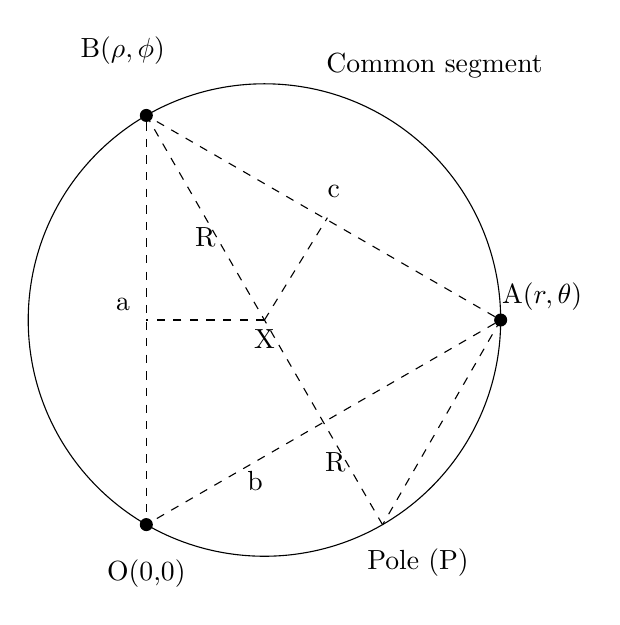
\begin{tikzpicture}

    % equidistant points and arc
    \foreach \x [count=\p] in {0,...,2} {
        \node[shape=circle,fill=black, scale=0.5] (\p) at (-\x*120:3) {};};
    \foreach \x [count=\p] in {0,1,2} {
        \draw (-\x*120:3.6);}
        /%\draw (-30-\x*60:3.6) node {$\bar{\p}$};}; 
    \draw (1) arc (0:360:3);
    \draw[dashed] (1) -- (2) node[pos=0.7, below]{b};
    \draw[dashed] (3) -- (2) node[pos=1.2, above]{O(0,0)};
    \draw[dashed] (1) -- (3);
    % axes
    \draw [dashed] (1.5,-2.6) -- (-1.5,2.6) node[pos=1.1, above]{B$(\rho,\phi)$} node[pos=-0.15, above]{Pole (P)} node[pos=0.2, below]{R} node[pos=0.75, below]{R};
    \draw [dashed] (0,0) -- (-1.5,-0.00) node[pos=1.2, above]{a};
    \draw [dashed] (0,0) -- (0.8,1.3) node[pos=1.1, above]{c} node[pos=2.7, below]{Common segment} node[pos=0, below]{X};
    \draw [dashed] (3,0) -- (1.5,-2.6) node[pos=-0.0, above]{\qquad \quad A$(r,\theta)$};
    
\end{tikzpicture}

\begin{align}
\vec{A} = \myvec{r\;\: sin(\theta)\\r \;\: cos(\theta)}, \;\: \nonumber \vec{B} =\myvec{\rho \;\:  sin(\phi)\\\rho \;\: cos(\phi)}, \nonumber
\end{align}
\begin{align}
\vec{O} =\myvec{0\;\: sin(0)\\0\;\: cos(0)} \nonumber
\end{align}
\begin{align}
\norm{\vec{A}-\vec{O}}^2 &= (\vec{A}-\vec{O})^\top (\vec{A}-\vec{O}) \nonumber \\
\norm{\vec{A-0}} &= \myvec{r\;\: sin(\theta)\\r \;\: cos(\theta)}, \nonumber \\
\vec{a} &= \myvec{r\;\: sin(\theta)\\r \;\: cos(\theta)}, \nonumber
\end{align}
\begin{align}
\norm{\vec{B}-\vec{O}}^2 &= (\vec{B}-\vec{O})^\top (\vec{B}-\vec{O}) \nonumber \\
\norm{\vec{B-0}} &= \myvec{\rho \;\:  sin(\phi)\\\rho \;\: cos(\phi)} \nonumber \\
\vec{b} &= \myvec{\rho \;\:  sin(\phi)\\\rho \;\: cos(\phi)} \nonumber
\end{align}\\
From the diagram, BP is diameter with X as circum-center of the triangle $\Delta OAB $.\\ \\
Also, $\Delta APB $ and $\Delta AOB $ share same segment. AB is same chord between them so by comparing both triangles,\\ \\
$\angle APB $ = $\angle AOB $,\\
From that we can say,
\begin{align}
\frac{c}{2R} = \frac{h}{a} \nonumber \\
\frac{c}{D} = \frac{h}{a} \\
In \;\: \Delta AOB,\;\: Area \:[AOB] &= \frac{1}{2}\;bh \nonumber \\ 
h &= \frac{2[AOB]}{b}
\end{align}
\begin{align}
Area \;\: [AOB] &= \frac{1}{2}\;ab\;\:sin(\theta)\nonumber \\ 
&= \frac{1}{2}\;\rho r\;\:sin(\theta-\phi)
\end{align}
From (1) and (2),
\begin{align}
\frac{c}{D} &= \frac{2[AOB]}{ab}\nonumber \\ \nonumber \\
abc &= 2D[AOB]\nonumber \\
2D &= \frac{abc}{[AOB]}
\end{align}
\begin{align}
c &= \sqrt{(r\:sin(\theta)-\rho\:sin(\phi))^2 + (r\:cos(\theta)-\rho\:cos(\phi))^2} \nonumber \\
&= \sqrt{r^2\:P + \rho^2\:P - 2\:r\rho\:(sin\theta\:sin\phi + cos\theta\:cos\phi)} \nonumber
\end{align}
\\
Where P is $(sin^2(\phi)-cos^2(\phi))$ which is 1 \\
and a = $\rho$ and b = $r$ \\
\begin{align}
c &= \sqrt{r^2 + \rho^2 - 2\:r\rho\: cos(\theta - \phi)}
\end{align}
From (4) and (5),
\begin{align}
2D &= \frac{\sqrt{r^2 + \rho^2 - 2\:r\rho\: cos(\theta - \phi) r \rho}}{\frac{1}{2}r \rho sin(\theta-\phi)} \nonumber \\
\vec{D} &= \frac{\sqrt{r^2 + \rho^2 - 2\:r\rho\: cos(\theta - \phi)}}{sin(\theta-\phi)}
\end{align}
\begin{figure}[!ht]
    \center
    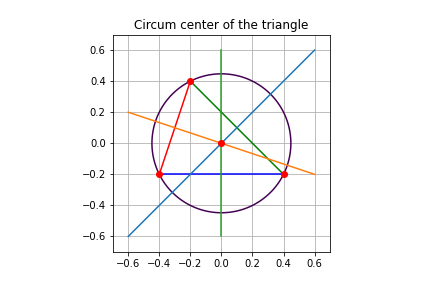
\includegraphics[width=300pt]{assignment_1.png}
    \label{fig:assignment-1}
\end{figure}
\end{document}